\chapter{Methodology}\label{chap:methodology}
This chapter details the methodologies employed in the development and evaluation of the RAG Chatbot and the low-rank approximation of the BART model. The aim is to provide a comprehensive understanding of the techniques, tools, and processes used to achieve the research objectives.

The chapter is structured into two main sections. The first section focuses on the RAG Chatbot, named Study Buddy, which was developed to assist students by providing detailed and context-specific responses. This section outlines the motivation for developing the chatbot, describes the tools and environment used, and explains the implementation steps taken to create the prototype. 
The second section addresses the low-rank approximation of the BART model. It describes how low-rank approximation was applied to the attention weight matrices of the BART model to reduce computational complexity and storage requirements while maintaining performance on summarization tasks. The implementation steps and evaluation metrics used to assess the effectiveness of this approach are also presented, along with the criteria for selecting an appropriate rank for computational efficiency and storage reduction.


\section{RAG Chatbot: Study Buddy}
    A survey conducted (by \cite{hanifi2023chatgpt}) reports that 93\% of software engineering students, comprising of mainly 3rd and 4th semester students, use ChatGPT during their course projects. Among them 80.2\% were categorized as active users which entails tasks as generating source code. A similar observation can be made by teaching assistants in the SW2PLA course at Aarhus University where students frequently resort to using chatbots like ChatGPT for quick answers to their questions. However, these chatbots often provide generic responses that may not be sufficiently helpful for academic purposes, as they lack the specificity and depth required for effective studying. This observation underscores a gap in the effectiveness of current chatbot solutions in educational contexts.

    The RAG model (\cite{lewis2020RAG}) addresses this gap by combining a retriever and a generator, thereby enabling the delivery of more detailed and context-specific information. 
    
    To gain practical experience with LLMs and their application in real-world language processing tasks, this thesis aims to develop a prototype for a chatbot inspired by a project at BSS - Aarhus University (Appendix \ref{appendix:Bergenholtz}). This chatbot, utilizises the RAG model \cite{lewis2020RAG}, serves as a 'Study Buddy' to assist students in understanding complex topics, providing quick and relevant answers, and enhancing their learning experience for challenging subjects.

    \subsection{Development and Environment Tools}
    The implementation of the RAG chatbot was accomplished using the following tools and technologies:
    \begin{itemize}
        \item \textbf{OpenAI API:} Utilized to access the GPT-4 model for the chatbot's generation capabilities.
        \item \textbf{Astra DB:} Employed for storing and managing the data used by the retriever component.
        \item \textbf{DataStax RAGstack:} A curated stack of leading open-source software designed to facilitate the implementation of the RAG pattern in production-ready applications using Astra Vector DB as a vector store.
        \item \textbf{Langchain:} An open-source framework used for developing applications powered by LLMs.
        \item \textbf{Streamlit:} An open-source Python framework used for building and deploying data applications with minimal code.
    \end{itemize}

    \subsection{Implementation Steps}
    The development of the RAG chatbot involves the following steps:
    \begin{enumerate}
        \item \textbf{Chatbot Interface:} Designing and creating a user-friendly interface for users to interact with the chatbot.
        \item \textbf{Generator Component:} Implementing the generator component to provide responses based on the GPT-4 model.
        \item \textbf{Retriever Component:} Developing the retriever component to search for relevant information in the AstraDB Vector Store based on user queries.
        \item \textbf{Integration:} Integrating the retriever and generator components to create a functional RAG chatbot.
        \item \textbf{PDF Uploader:} Implementing a feature that allows users to upload their own materials, enabling more meaningful and contextual responses.
        \item \textbf{Deployment:} Deploying the chatbot on a cloud platform to make it possible to be publicly accessible.\footnote{As the current implementation of the chatbot uses a private OpenAI account and due to the costs associated with this, the current implementation of the chatbot is not publicly accessible. However, access can be provided upon request.}

    \end{enumerate}
        
    The conceptual workflow of the Study Buddy, is depicted in Figure \ref{fig:rag_architecture}, where in Studdy Buddy's case AstraDB is used as the knowledge source and OpenAI's ChatGPT-4 as generator. The process begins with the user inputting a query, which is then processed by the retriever to find relevant information. This information provides context based on the user's query. Subsequently, the generator creates a response using an embedded prompt template, the retrieved information, and the user's query, thereby providing the user with a detailed and specific answer.



\section{Case Study: Low-Rank Approximation of BART model}
    To assess the effectiveness of low-rank approximation in compressing Facebook's BART-model (\cite{lewis2019bart}), both its base- and large model versions are considered as a case study.

    This thesis focuses on applying low-rank approximation specifically to the attention matrices. This choice stems from their pivotal role in the transformer architecture \cite{vaswani2023attention}. These matrices, which help the model assess the relevance of different words within the input data, tend to be large and often encapsulate redundant information (\cite{aghajanyan2020intrinsic}).

    By applying low-rank approximation to the attention weight matrices of the BART model, the possibility of reducing computational complexity and storage requirements while preserving performance on a summarization task is explored.

    \subsection{Implementation Steps}
        The implementation of low-rank approximation for BART involves the following steps:
        \begin{enumerate}
            \item \textbf{Computing SVD of Attention Weight Matrices:} The attention weight matrices (Key, Query, Value, and Output) of the model are decomposed using SVD to obtain the low-rank approximation.
            \[
            \begin{array}{c}
                Q \\[0.2cm] % adds 0.5 cm space after this row
                V \\[0.2cm] % adds 0.5 cm space after this row
                K \\[0.2cm]
                O
            \end{array}
            \xrightarrow[\text{SVD}]{\hspace*{1cm}}
            \begin{array}{c}
                U_q \ \Sigma_q \ V_q^T \\[0.2cm] % adds 0.5 cm space after this row
                U_v \ \Sigma_v \ V_v^T \\[0.2cm] % adds 0.5 cm space after this row
                U_k \ \Sigma_k \ V_k^T \\[0.2cm]
                U_o \ \Sigma_o \ V_o^T

            \end{array}
            \]

            \item \textbf{Custom Layer Implementation:} A custom layer is implemented to replace the original attention layers with the low-rank approximation.
            \begin{figure}[H]
                \centering
                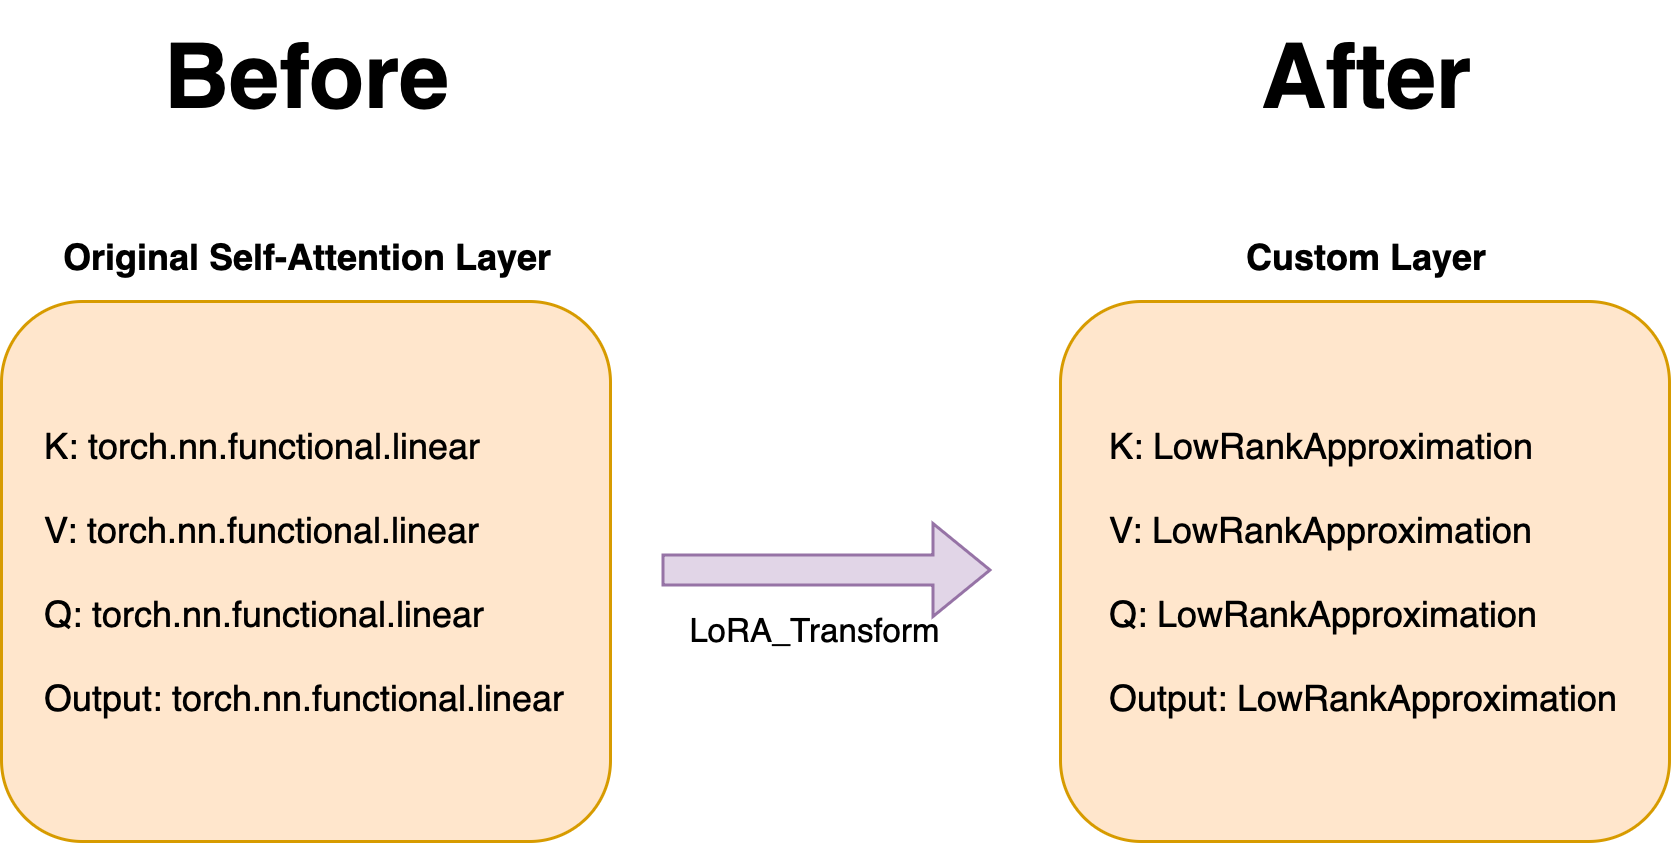
\includegraphics[width=0.7\textwidth]{figs/before-after.png}
                \caption{Components in attention layers replaced with their custom low-rank approximation}
                \label{fig:lora_implementation}
            \end{figure}
        \end{enumerate}
        
        
        
    \subsection{Evaluation Metrics}\label{sec:evaluation_metrics}
        The approximated model is evaluated based on:
        \begin{enumerate}
        \item ROUGE scores (\cite{lin-2004-rouge}): How well does the approximated model perform in comparison to the original BART-Base/Large model on the summarization task? From which rank does the model start to lose performance?
        \item Computational efficiency: How does the approximated model compare to the original BART-Base/Large model in terms of computational resources required?
        \item Comparing some of the summaries generated by the compressed model with the original BAR-Base/Large model and the reference summaries using the Samsum dataset (\cite{gliwa-etal-2019-samsum}).
        \begin{figure}[H]
            \centering
            \includegraphics[width=0.6\textwidth]{figs/dialogue.png}
            \caption{SamSum Dataset \texttt{test[0]} dialogue and reference summary}
            \label{fig:SamSum_Example}
        \end{figure}
        \end{enumerate}

        \subsection{Appropriate Rank Selection}
            In section \ref{sec:reduction_storage}, the criterion for selecting an appropriate rank \(k\) to achieve computational efficiency and storage reduction is established. The criterion is given by:
            
            \[
            k < \frac{\sqrt{4mn + (m+n)^2} - m - n}{2}
            \]
            
            where \(m\) and \(n\) are the dimensions of the original matrix to be approximated with a low-rank representation.
            
            \textbf{BART-base Model:}\\
            For the BART-base model, the attention matrices have dimensions \(m = n = 768\). This can be verified by inspecting the model's architecture (Appendix \ref{appendix:BART}).\\
            Therefore, the rank \(k\) for the approximation should satisfy:
            \[
            k < \frac{\sqrt{4 \times 768 \times 768 + (768 + 768)^2} - 768 - 768}{2} \approx 318
            \]
            
            \label{appropriate_rank}to achieve a reduction in computational complexity and storage requirements.

            \textbf{BART-large Model:}\\
            Similarly, for the BART-large model, the attention matrices have dimensions \(m = n = 1024\). Therefore, the rank \(k\) for the approximation should satisfy:
            \[
            k < \frac{\sqrt{4 \times 1024 \times 1024 + (1024 + 1024)^2} - 1024 - 1024}{2} \approx 424
            \]
            To determine the feasibility of low-rank approximation for the two BART models, the approximated model at various ranks will be evaluated and then the impact on the ROUGE scores will be observed. This evaluation will illucidate the trade-offs between rank reduction and model performance in the specific case of BART.

